\apendice{Plan de Proyecto Software}

\section{Introducción}

En este apartado se pretende exponer la planificación y viabilidad del proyecto. Se mostrará el avance temporal del proyecto, los avances que tuvieron lugar entre cada reunión y el estudio de viabilidad económica y legal.

\section{Planificación temporal}

Se ha intentado seguir la metodología Agile, utilizando \textit{\textit{sprints}} o bloques de trabajo de unas dos semanas. En ocasiones por circunstancias de trabajo, vacaciones o imposibilidad los \textit{sprints} se han prolongado durante 1 mes. Además hubo una interrupción del proyecto entre el \textit{sprint} 7 y 8 por cuestiones laborales y personales del autor/alumno. 

El trabajo no se ha realizado de forma homogénea en todos los \textit{sprints}. Durante los períodos vacacionales (verano y navidad) se ha realizado la mayor parte del desarrollo, y en los meses anteriores al depósito de la memoria se avanzó la mayor parte de la escritura y documentación del proyecto.

Tras cada \textit{sprint} se mantenía una reunión entre los tutores y alumno, en la cual se debatían los avances y se planificaba en qué se iba a trabajar en el siguiente sprint.

\subsection{Sprint 1 - 27/06/23 a 5/07/23}

En este \textit{sprint} se hizo un primer estudio de la viabilidad del proyecto y se decidieron las tecnologías a utilizar según la idea propuesta originalmente. Además se hizo un prototipo del \textit{scraper}.

\begin{itemize}
    \item Se comprobó que la página web \url{www.idealista.com} estaba totalmente protegida contra el \textit{scraping}. Tras solicitar una clave para \textit{API} que permitiera el desarrollo del proyecto no se obtuvo respuesta por parte de idealista.

    Por tanto, se decidió que la fuente de los datos iba a ser \url{www.pisos.com}, otro portal inmobiliario de los más grandes de España y que no bloquea el uso de \textit{scraping}.
    \item Se hizo un diagrama de las tecnologías que se pretendían usar para la fase de extracción, transformación, carga de los datos y su análisis mediante \textit{Machine Learning}, además de la orquestación de los distintos procesos.
    \item Se probaron diversas tecnologías de \textit{scraping}, para finalmente decidir usar scrapy.
    \item Se desarrolló un prototipo de \textit{scraper} para inmuebles en venta en \url{www.pisos.com}.
\end{itemize}

\subsection{Sprint 2 - 05/07/23 a 29/08/23}

En este sprint, algo más largo por las fechas vacacionales, se logró un gran avance en la parte de desarrollo.

\begin{itemize}
    \item Se amplió el software de \textit{scraping}, pasando a recopilar más de 50 datos por inmueble.
    \item Se diseñó y desplegó la base de datos primaria que almacenaría la ingestión de datos proveniente de \textit{scraping}: MongoDB.
    \item Se desplegó una máquina virtual Ubuntu alojada en Oracle \textit{cloud}, en la cual se empezaron a recoger datos diariamente.
    \item Se estableció un mecanismo de \textit{backup} de la base de datos primaria en caso de catástrofe en la máquina virtual del proyecto.
    \item Se comenzó a esbozar el procedimiento de ETL de datos \textit{raw} almacenados en la MongoDB.
\end{itemize}

\subsection{Sprint 3 - 29/08/23 - 13/09/23}

En este sprint, se desplegó el proceso de ETL.

\begin{itemize}
    \item Finalización del diseño y decisión de las tecnologías aplicadas en el proceso de ETL.
    \item Se desplegó el proceso de ETL, en Python, que recoge los datos en crudo de la MongoDB, los transforma y los carga, en una base de datos relacional: SQLlite.
    \item Se hicieron algunas exploraciones previas de los datos limpios.
\end{itemize}

\subsection{Sprint 4 -  13/09/23 - 26/09/23}

Este \textit{sprint} se dedicó a la puesta al día de la documentación del proyecto. Además se desplegó Apache Airflow como orquestador, debido al previsible aumento de complejidad de los procesos.

\begin{itemize}
    \item Despliegue de Apache Airflow como orquestador.
    \item Puesta al día de la documentación y memoria de los \textit{sprints} 1, 2, 3 y 4.
\end{itemize}

\subsection{Sprint 5 -  26/09/23 - 10/10/23}

Este \textit{sprint} se dedicó a finalizar la puesta al día de la documentación del proyecto.

\begin{itemize}
    \item Puesta al día de la documentación y memoria de los \textit{sprints} 1, 2, 3 y 4.
\end{itemize}

\subsection{Sprint 6 -  10/10/23 - 24/10/23}

En este \textit{sprint} se comenzó el análisis de los datos provenientes de la ingestión. Se realizó un análisis exploratorio en Jupyter Notebook

\begin{itemize}
    \item Análisis exploratorio de los datos en la base de datos relacional utilizando Jupyter Notebooks.
    \item Esbozo del problema a resolver mediante ciencia de datos.
\end{itemize}


\subsection{Sprint 7 -  24/10/23 - 07/11/23}

En este \textit{sprint} se exploraron los modelos de \textit{\textit{\textit{Machine Learning}}} a utilizar y el proceso de entrenamiento de dichos modelos.

\begin{itemize}
    \item Iteraciones de entrenamiento y predicción con modelos de la libreria Scikit-Learn para intentar resolver el problema de asignar una puntuación a inmuebles.
    \item Pruebas de entrenamiento y predicción con todo el conjunto de datos en el entorno de Jupyter Notebooks.
\end{itemize}

\subsection{Proyecto parado -  07/11/23 - 07/12/23}

Por motivos laborales y personales en este período de tiempo no se pudo avanzar en el proyecto.

\subsection{Sprint 8 -  07/12/23 - 19/12/23}

En este \textit{sprint} se creó el esqueleto de la web de visualización de los datos.

\begin{itemize}
    \item Creación de esqueleto \textit{frontend} funcional con React.
    \item Creación de servidor \textit{backend} funcional con Node.js y ExpresS que conecta con la base de datos de producción SQLite.
\end{itemize}

\subsection{Sprint 9 -  19/12/23 - 02/01/24}

En este \textit{sprint} se arreglaron defectos en el proceso de ingestión de datos. Además, se añadieron nuevas funcionalidades a dicho proceso de ingestión de datos. Por otra parte, se desplegó el servicio de \textit{\textit{Machine Learning}}. Finalmente, se continuaron añadiendo funcionalidades a la web.

\begin{itemize}

    \item Se arregló un defecto que hacía que un único inmueble (y por tanto una única clave primaria) estuviera duplicada en la base de datos secundaria. El error se producía cuando un inmueble había estado listado en distintas ciudades (y por tanto se ingestaba en distintas colecciones de la base de datos MongoDB).
    \item     Se implementó en el servicio de \textit{scraping} una comprobación de si el inmueble sigue activo. Tanto dentro de la base de datos primaria (MongoDB) como secundaria (SQLite) el inmueble se marca si está activo o no.
    \item Se desplegó el proceso de entrenamiento de los modelos de \textit{Machine Learning}.
    \item Se desplegó el proceso que asignaba una puntuación a los inmuebles ya existentes y a todos los nuevos que se fuesen introduciendo, utilizando los modelos previamente mencionados.
    \item Se continuó el desarrollo de funcionalidades del sitio web donde se muestran los datos y puntuaciones de los inmuebles.
    \item Se dio por concluida la parte del proyecto de ingeniería y ciencia de datos, salvo por retoques finales.
\end{itemize}

\subsection{Sprint 10 -  02/01/24 - 16/01/24}

Durante este \textit{sprint} se hizo un esfuerzo por mejorar el entorno DevOps del proyecto mediante el uso de contenedores de software con la tecnología Docker. El proyecto quedó desplegado en una máquina virtual de Oracle Cloud con Sistema Operativo Ubuntu en la que se desplegaron dichos contenedores. El proyecto se consideró operativo a falta de finalizar el desarrollo de la web de análisis y visualización de datos y finalizar la documentación.

\begin{itemize}
    \item Creación de un contenedor Docker para el servicio de Scrapy.
    \item Creación de un contenedor Docker para los servicios de ETL.
    \item Creación de un contenedor Docker para los servicios de \textit{Machine Learning} (Entrenamiento y Predicción).
    \item Creación de un contenedor Docker para la MongoDB.
    \item Creación de un contenedor Docker para Airflow Webserver y otro para Airflow Scheduler.
    \item Creación de un contenedor Docker para el \textit{frontend} y otro para el \textit{backend} de los servicios web.
    \item Creación de volúmenes docker para almacenamiento permanente de logs, base de datos secundaria (SQLite), base de datos primaria (mongodb) y \textit{logs} y datos de Apache Airflow.
    \item Orquestación y despliegue de los contenedores utilizando Docker Compose.
    \item Puesta al día de la documentación y memoria de los \textit{sprints} 6, 7, 8, 9 y 10.
\end{itemize}

\subsection{Sprint 11 -  16/01/24 - 30/01/24}

En este \textit{sprint} se detectaron cambios en la web \url{www.pisos.com} que afectaron significativamente al flujo de datos ya que el \textit{scraping} dejó de funcionar. Supuso un rediseño del módulo de \textit{scraping}.

Además se rediseñó la agrupación geográfica de pisos para que fuera más consistentes. Por último se añadió un nuevo parámetro a todo el flujo de datos: Si in inmueble pertenecía a la capital o no.

Se avanzó significativamente en el \textit{frontend} de la web, tanto en la parte de funcionalidades como en la estética.


\begin{itemize}
    \item El módulo de \textit{scraping} se adaptó a la nueva web de \textit{www.pisos.com}.
    \item El script que comprobaba si un inmueble seguía activo se adaptó a la nueva web de \textit{www.pisos.com}.
    \item Se reorganizaron las colecciones de la base de datos MongoDB, para que coincidieran con las provincias de españa.
    \item El proceso de ETL crea un nuevo parámetro que indica si el inmueble pertenece a la capital de provincia o no.
    \item El proceso de agregación de datos ahora tiene en cuenta las provincias y si es capital de provincia o no.
    \item El proceso de entrenamiento y predicción de Aprendizaje Automático ahora tiene en cuenta las provincias como agrupación territorial y tiene en cuenta si el inmueble es capital o no.
    \item Se adaptó el \textit{backend} de la web para filtrar por provincias y si el inmueble es capital o no.
    \item Añadidas todas las funcionalidades principales a las vistas de la web: ``INICIO'', ``EXPLORA'', ``VISUALIZA'' e ``INFO''.
    \item Se mejoró la estética de la web.
\end{itemize}

\subsection{Sprint 12 -  30/01/24 - 13/02/24}

En este \textit{sprint} se continuó con la escritura de la memoria del proyecto y la revisión de cambios propuestos por tutor y co-tutor. Además se corrigieron algunos \textit{bugs} detectados en la web y se mejoraron algunos aspectos de la interfaz de usuario señalados por los revisores.

\begin{itemize}
    \item Arreglado bug en pestaña ``VISUALIZA''. No se estaban haciendo la media de las comunidades autónomas, se estaba asignado el valor de la primera provincia de esa comunidad autónoma (por orden alfabético).
    \item Mejorado comportamiento de filtros en pestaña ``EXPLORA''. Más intuitivos y fácil de seleccionar rango, solo se actualiza el estado cuando el usuario deja de arrastrar el selector. Añadido comportamiento de \textit{scroll} infinito en el listado de inmuebles.
     \item Agregada pestaña de información en puntuaciones y selector de modo. ``Inteligente'' en pestaña ``INICIO''
     \item Añadidas leyendas, títulos y unidades a gráficos de líneas.
     \item Añadida página de \textit{landing} en pestaña ``INICIO''
     \item Mejorado comportamiento de la web en dispositivos móviles
     \item Creado dominio \href{https://www.buscahogar.es}{buscahogar.es} y creado auto renovado de certificado https
\end{itemize}

\subsection{Sprint 13 -  13/02/24 - 22/02/24}

En este \textit{sprint} se finalizó la escritura de la memoria del proyecto y la revisión por parte del tutor y co-tutor. Además, se retocaron algunos aspectos visuales menores de la web. Se reestructuró código para hacerlo más mantenible.

\clearpage
\section{Estudio de viabilidad}

En esta sección se va a desarrollar cómo de viable ha resultado el desarrollo del proyecto a nivel económico y legal. 

\subsection{Viabilidad económica}

Se ha decidido desglosar la viabilidad económica en apartados de personal, infraestructura en la nube y hardware. Finalmente se mostrará el sumatorio.

\subsubsection{Coste Personal}

El proyecto se ha llevado a cabo por un desarrollador autónomo contratado durante 225 horas. Se considera un coste por hora de 40€ antes de IVA.

\begin{table}[!ht]
	\centering
	\begin{tabular}{lrrr}
		\toprule
		\textbf{Concepto} & \textbf{Coste/h} & \textbf{Horas} & \textbf{Coste Acumulado} \\
		\midrule
		Salario bruto & 40€ & 225 & 9000€\\
		IVA (21\%) & 8.4€ & & 1890€ \\
		\midrule
		\textbf{Total Proyecto} & & & 10\,890€ \\
		\bottomrule
	\end{tabular}
	\caption{Costes de personal desarrollador}
	\label{tab:personal}
\end{table}


\subsubsection{Coste Infraestructura y hardware - Prueba de concepto actual}

Uno de los mayores hitos de este proyecto es que se ha enmarcado todo en una sola máquina virtual de tipo \texttt{VM.Standard.A1.Flex}, con 24GB de RAM y 100GB de almacenamiento. Esta máquina es proporcionada indefinidamente de forma gratuita por \textit{Oracle Cloud}, por lo que el coste real de infraestructura la prueba de concepto ha sido de \textbf{0€} a lo largo de 8 meses. 

En el caso de que no se tuviera acceso a esta promoción y como ejercicio para estudiar la viabilidad del proyecto podemos estimar el cálculo de una máquina similar en el proveedor de \textit{Amazon Web Services o AWS}. Se ha estimado el coste de una máquina similar a la usada,  \textit{EC2 m6g.xlarge} (Ver Figura \ref{fig:ec2_costs}). A este coste  habría que sumar gastos de almacenamiento~\cite{ebs_pricing}. La suma de costes se puede ver en Tabla \ref{tab:infraestructura_aws}


\begin{figure}[ht]
    \centering
	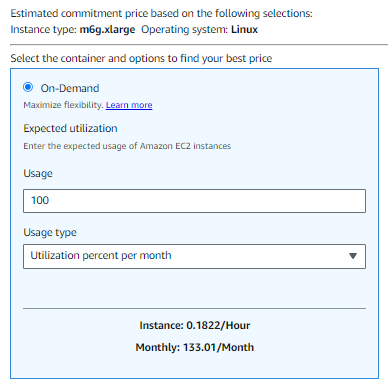
\includegraphics[width=0.8\textwidth]{img/ec2_cost.PNG}
	\caption[Coste del servicio de computación en la nube (EC2) de AWS para una máquina \textit{m6g.xlarge}]{Coste del servicio de computación en la nube (EC2) de AWS para una máquina \textit{m6g.xlarge}  (4 núcleos y 16GB de ram). Coste a día 8 febrero de 2024 para región EU (Spain).}
	\label{fig:ec2_costs}
\end{figure}


\begin{table}[!ht]
	\centering
	\begin{tabular}{lrrr}
		\toprule
		\textbf{Concepto} & \textbf{Coste/mes} & \textbf{Meses} & \textbf{Coste Acumulado} \\
		\midrule
		EC2 m6g.xlarge & 133\$ & 8 & 1064\$\\
        EB2 storage (100gb) & 8\$ & 8 & 64\$\\
		\midrule
        IVA (21\%) & & & 236\$ \\
		\midrule
		{Total Proyecto en \$} & & & 1364\$ \\
        \midrule
		\textbf{Total Proyecto en €} & Ratio \$ a € de 0.93 & & 1\,466€ \\
		\bottomrule
	\end{tabular}
	\caption{Costes de infraestructura en \textit{cloud} - Estimados para AWS}
	\label{tab:infraestructura_aws}
\end{table}


\begin{table}[!ht]
	\centering
	\begin{tabular}{lrrrr}
		\toprule
		\textbf{Concepto} & \textbf{Coste} & \textbf{Amortizado/mes} & \textbf{Meses} & \textbf{Total} \\
		\midrule
		Portátil & 1500€ & 31.25€  & 8 & 250€\\
        Periféricos & 300€ & 6.25€  & 8 & 50€\\
        Monitores & 300€ & 6.25€  & 8 & 50€\\
        Silla y escritorio & 500€ & 10.42€  & 8 & 83.36€\\
        \midrule
		\textbf{Total Proyecto} & & & & 433.36€ \\
		\bottomrule
	\end{tabular}
	\caption[Costes de hardware]{Costes de hardware. Para el cálculo de coste mensual, se ha considerado un período de amortización de 48 meses para el coste total del producto.}
	\label{tab:hardware}
\end{table}


\subsubsection{Coste total del proyecto}

En la tabla \ref{tab:coste_total} se muestra la suma de los costes de personal, infraestructura en la nuble y hardware, mostrados en subsecciones anteriores.

\begin{table}[!ht]
	\centering
	\begin{tabular}{ll}
		\toprule
		\textbf{Concepto} & \textbf{Coste } \\
		\midrule
		Personal & 10\,890€\\
        Infraestructura Cloud &  1\,466€\\
        Hardware y accesorios & 433€\\
        \midrule
		\textbf{Total Proyecto} &  12\,789€ \\
		\bottomrule
	\end{tabular}
	\caption{Coste total del proyecto (8 meses).}
	\label{tab:coste_total}
\end{table}

\subsection{Viabilidad legal}

En este subapartado se muestran las licencias que tienen las herramientas y librerías usadas (Ver tabla~\ref{tab:dependencias}). Siguiendo las recomendaciones GNU~\cite{gnu}, se ha escogido la licencia GPL-3.0~\cite{gpl3} para el presente proyecto. Esta licencia permite la modificación, uso y distribución del software, siempre que se realice bajo la misma licencia, se indiquen los cambios y se mencione al autor original.

Por último, durante este proyecto, se ha comprobado que el uso de \textit{scraping} en el portal \url{www.pisos.com} se trata de un proceso legal y ético, ya que se cumple en su totalidad las recomendaciones especificadas por la página web en su archivo ``robots.txt''~\cite{pisosrobotstxt}. Además se han seguido prácticas de limitación de número de peticiones diarias, para no suponer una sobrecarga a los servidores de dicho portal.


\begin{table}[h]
	\centering
	\begin{tabular}{@{}ll@{}}\toprule
		\textbf{Dependencia}         & \textbf{Licencia}     \\ \midrule
		\textbf{Librerías Python} & \\
        Scrapy               & BSD \\
        Pandas               & BSD-3-Clause \\
        Numpy                & BSD \\
		Pymongo              & Apache License 2.0 \\
  	Scikit-learn         & BSD \\
		Scipy                & BSD \\
        Matplotlib           & Python Software Foundation License \\
        \midrule
        \textbf{Librerías Web} & \\
        React                & MIT \\
		Node.js              & MIT \\
        Express              & MIT \\
        Cors                 & MIT \\
		Dotenv               & MIT \\
		Pg                   & MIT \\
		Sqlite3              & MIT \\
        MUI                  & MIT \\
		Axios                & MIT \\
		Bootstrap            & MIT \\
		Leaflet              & BSD \\
		Recharts             & MIT \\
        \midrule
        \textbf{Herramientas} & \\
		MongoDB              & Server Side Public License (SSPL) \\
		Apache Airflow       & Apache License 2.0 \\
		Nginx                & BSD de 2 cláusulas \\
        \bottomrule
	\end{tabular}
	\caption{Tabla de dependencias del proyecto}
	\label{tab:dependencias}
\end{table}

